\documentclass[pdf]{beamer}
\usepackage[french]{babel}
\usepackage{graphicx}
\usetheme{Rochester}
\usecolortheme{whale}

\title{Développez un programme logiciel en Python}
\subtitle{OpenClassRooms - Parcours Python - Projet 4}
\author{Bérenger Ossété Gombé}

\begin{document}
\begin{frame}
  \titlepage
\end{frame}

\AtBeginSection[]{
  \begin{frame}{Rappel du sommaire}
    \setcounter{tocdepth}{2}
    \tableofcontents[currentsection, hideothersubsections]
  \end{frame}
}

\begin{frame}{Sommaire}
  \setcounter{tocdepth}{65536}
  \tableofcontents
\end{frame}

\section{Introduction}
\begin{frame}{Présentation}

  \begin{center}
    
\includegraphics[scale=0.5]{img/logo_ufc.png}
    \hspace{1em}
    
\includegraphics[scale=0.3]{img/logo_ocr.png}
  \end{center}
  
  \begin{block}{Bérenger Ossété Gombé}
    \begin{itemize}
    \item Master 1 en informatique (2016-2017)
      \begin{itemize}
      \item Université de Franche-Comté (UFR-ST)
      \item Spécialité génie logiciel
      \end{itemize}
    \item Formation Python chez OpenClassRooms depuis janvier 2022
    \end{itemize}    
  \end{block}
\end{frame}

\begin{frame}{Le Projet n°4: développer un programme logiciel en Python}

  \begin{block}{Objectifs}
    \begin{itemize}
    \item Produire du code robuste
    \item Utiliser la POO
    \item Structurer un projet python
    \end{itemize}
  \end{block}
\end{frame}

\begin{frame}{Contexte fictif: le club d'échecs}
  \begin{figure}
    \begin{center}
      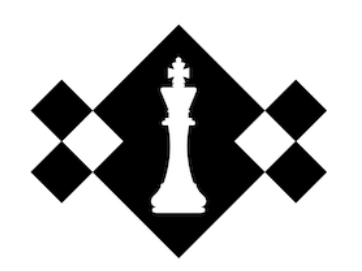
\includegraphics[scale=0.2]{img/logo_club.png}    
    \end{center}    
    \caption{Logo du club d'échecs}    
  \end{figure}
  
  \begin{block}{Personnages}
    \begin{itemize}
    \item Nous incarnons un développeur indépendant
    \item Quelques membres du club d'échecs
      \begin{itemize}
      \item Élie, notre amie
      \item Édouard, l'oganisateur
      \item Charlie, l'assistant informatique
      \end{itemize}
    \end{itemize}
  \end{block}
\end{frame}

\begin{frame}{Contexte fictif: le club d'échecs}
  \begin{block}{Problématique}
    \begin{itemize}
    \item «\textit{Nous utilisons actuellement une \textbf{application
        en ligne} pour nous aider à gérer nos tournois d'échecs
      hebdomadaires. Malheureusement, cette application nous a déçus par
      le passé. Elle \textbf{tombe souvent en panne}, ce qui signifie
      que les matchs sont retardés.}» - \underline{Spécification technique}

    \item «\textit{Après que nous avons eu terminé le premier tour,
      \textbf{Internet a cessé de fonctionner} et le directeur du tournoi n'a
      pas pu entrer les scores sur le site des résultats}» - \underline{Témoignage d'Élie}
    \end{itemize}
  \end{block}
\end{frame}

\begin{frame}{Le besoin client}
  \begin{block}{Exigences fonctionnelles}
    \begin{itemize}
    \item Gestion des tournois
    \item Gestion des classements
    \item Génération de rapports pouvant être exportés\footnote{Il faut permettre cette future fonctionnalité.}
    \item Fonctionnement hors-ligne
    \item Interaction utilisateur \textit{via} une interface console
    \item Persistance \textit{via} une base de données
    \end{itemize}
  \end{block}
\end{frame}

\begin{frame}{Le besoin client}
  \begin{block}{Exigences non-fonctionnelles \footnote{Extraites de la spécification technique.}}
    \begin{itemize}
    \item \textbf{Maintenabilité}
      \begin{itemize}
      \item «\textit{Le code doit être \underline{aussi propre et maintenable que
        possible} pour éviter les bugs.}»
      \end{itemize}
    \item \textbf{Fiabilité}
      \begin{itemize}
      \item «\textit{Le code doit être aussi propre et maintenable que
        possible pour \underline{éviter les bugs}.}»
      \end{itemize}

    \item \textbf{Portabilité} (GNU/Linux, Windows, MacOS)
      \begin{itemize}
      \item «\textit{Le programme devrait fonctionner sous
        \underline{Windows, Mac ou Linux}}»
      \end{itemize}

    \item \textbf{Utilisabilité}
      \begin{itemize}
      \item «\textit{Tant que le programme affiche les résultats du
        tournoi \underline{proprement}, nous serons heureux !}»
      \end{itemize}      
    \end{itemize}
  \end{block}
\end{frame}


\section{Méthodes et outils}
\subsection{Agilité et tests}
\begin{frame}{Agilité}
  \begin{block}{Mise en place du backlog}
    \begin{itemize}
    \item Utilisation d'un tableau Kanban \textit{via} kanboard \footnote{\url{https://kanboard.org/}}
    \item Découpage des \textit{user stories} avec critères d'acceptations
    \end{itemize}
  \end{block}
\end{frame}

\begin{frame}{Tests}
  \begin{block}{Pourquoi tester ?}
    \begin{itemize}   
    \item La fiabilité est un enjeu du projet
      \begin{itemize}
      \item «\textit{Le code doit être aussi propre et maintenable que
        possible \textbf{pour éviter les bugs}.}»\footnote{D'après la
      spécification technique.}
      \end{itemize}
    \item L'algorithme du tournoi Suisse doit être fiable car au cœur
      du domaine métier
    \end{itemize}
  \end{block}
  
  \begin{block}{Outils de tests}
    \begin{itemize}
    \item Tests unitaires \textit{via} PyTest \footnote{\url{https://docs.pytest.org/en/7.1.x/}}
    \item Tests d'acceptations \textit{via} Behave
      (cucumber) \footnote{\url{https://behave.readthedocs.io/en/stable/}}
    \end{itemize}    
  \end{block}
\end{frame}

\subsection{Style et conventions}
\begin{frame}{Style et conventions}
  \begin{block}{PEP 8}
    \begin{itemize}
    \item Vérification de la conformité du programme avec PEP 8
      \textit{via}
      Flake8\footnote{\url{https://flake8.pycqa.org/en/latest/}}
    \end{itemize}
  \end{block}
  
  \begin{block}{Google et OpenStack}
    \begin{itemize}
    \item Google Python Style Guide \footnote{\url{https://google.github.io/styleguide/pyguide.html}}
    \item OpenStack Style
      Guidelines \footnote{\url{https://docs.openstack.org/hacking/latest/user/hacking.html}}
    \item Utilisation de l'extension
      hacking\footnote{\url{https://pypi.org/project/hacking/}} de
      Flake8
    \end{itemize}
  \end{block}
\end{frame}

\subsection{Bibliothèques Python}
\begin{frame}{Bibliothèques Python}
  \begin{block}{Bibliothèques}
    \begin{itemize}
    \item Style et conventions
      \begin{itemize}
      \item Flake8
      \item Flake8-html
      \item Hacking      
      \end{itemize}

    \item Tests
      \begin{itemize}
      \item PyTest
      \item Behave
      \end{itemize}

    \item Base de données
      \begin{itemize}
      \item TinyDB
      \end{itemize}
    \end{itemize}
  \end{block}
\end{frame}


\section{Modélisation objet}
\subsection{Conception et modélisation}

\begin{frame}{Vocabulaire: traductions}
  \begin{block}{Traduction en anglais du vocabulaire}
    \begin{description}
    \item[Tournoi] \textit{tournament}
    \item[Classement] \textit{ranking}
    \item[Rapport] \textit{report}
    \item[Joueur] \textit{player}
    \item[Pair de joueur] \textit{pair of players}
    \item[Un tour] \textit{a round}
    \item[Résultats] \textit{scores}
    \item[Match nul] \textit{draw}
    \end{description}
  \end{block}
\end{frame}

\begin{frame}{Découpage en modules}
  \begin{block}{Modèle MVC}
    \begin{itemize}
    \item un modèle (\textit{package} \textsc{model})
    \item une vue (\textit{package} \textsc{view})
    \item un contrôleur (\textit{package} \textsc{controller})
    \end{itemize}
  \end{block}
\end{frame}

\begin{frame}{Architecture}
  \begin{block}{Propriétés}
    \begin{enumerate}
    \item Indépendance du modèle vis-à-vis du contrôleur et de la vue.
    \item Le contrôleur est le point central de l'architecture.
    \item La vue et le modèle communiquent \textit{via} des
      évènements.
    \end{enumerate}
  \end{block}  
\end{frame}

\begin{frame}{Architecture}
  \begin{center}
    \begin{figure}
      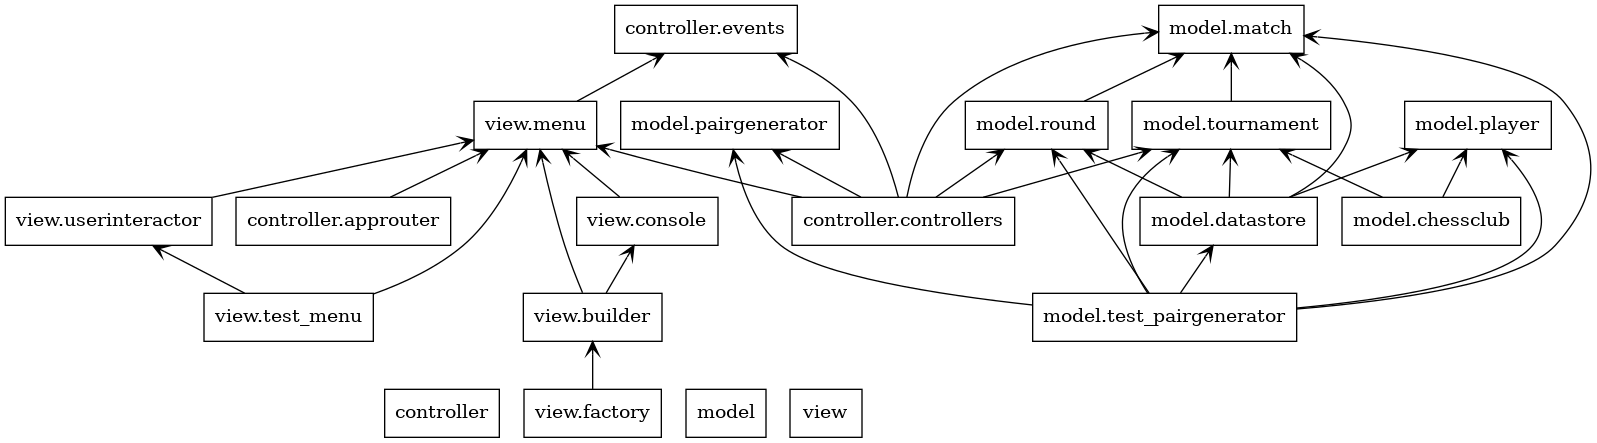
\includegraphics[scale=0.205]{img/architecture.png}
      \caption{Les \textit{packages}}
    \end{figure}
  \end{center}
\end{frame}

\begin{frame}{Le modèle}
  \begin{center}
    \begin{figure}
      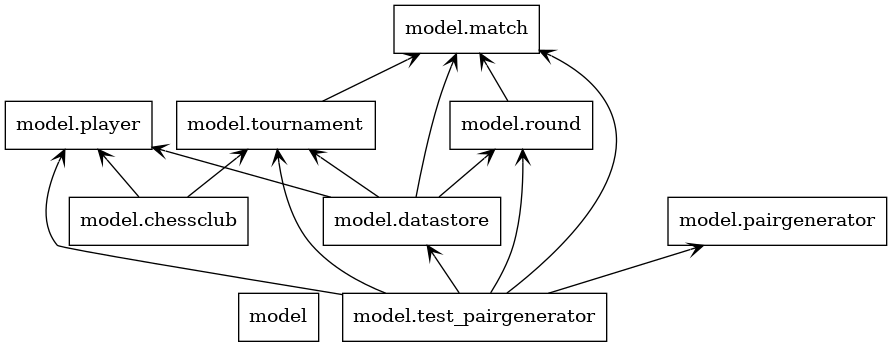
\includegraphics[scale=0.25]{img/model.png}
      \caption{Structure du modèle}
    \end{figure}
  \end{center}

  \begin{block}{Remarque}
    \begin{itemize}
    \item \textsc{ChessClub} implémente le \textit{design pattern
      Facade}.
    \end{itemize}
    
  \end{block}
\end{frame}

\begin{frame}{La vue}
  \begin{center}
    \begin{figure}
      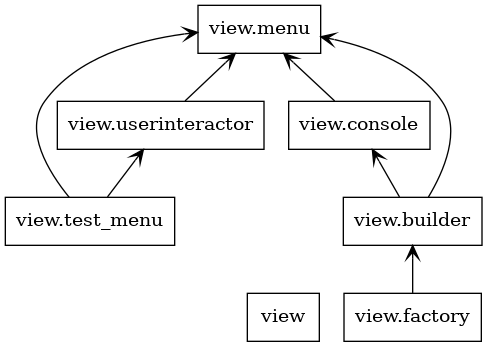
\includegraphics[scale=0.3]{img/view.png}
      \caption{Structure de la vue}
    \end{figure}
  \end{center}

  \begin{block}{Construction de la vue}
    \begin{itemize}
    \item La \underline{\textit{factory}}
      \begin{itemize}
      \item permet de charger la description XML de la vue.
      \item utilise un \underline{\textit{Builder}} pour construire la vue.
      \end{itemize}
    \end{itemize}
  \end{block}
\end{frame}

\begin{frame}[fragile]{La vue: représentation XML}
  \small

  \begin{minted}{xml}
    <menu title='Menu Principal'>
        <entry action='S'>Sauvegarder</entry>
        <entry action='C'>Charger</entry>

        <menu title="Rapports" action="R">
        <entry action='a'>Acteurs (par nom)</entry>
        <entry action='A'>Acteurs (par classement)</entry>
        <entry action='t'>Tournoi (acteurs par nom)</entry>
        <entry action='T'>
            Tournoi (acteurs par classement)
        </entry>
        <entry action='l'>Liste des tournois</entry>
        <entry action='L'>Liste des tours</entry>
        <entry action='m'>Liste des matchs</entry>
        <link action='q'>Menu Principal</link>
        </menu>

        <!-- ... -->
    </menu>
  \end{minted}
\end{frame}

\begin{frame}[fragile]{Événements}
  \footnotesize
  \begin{minted}{python}
class Event:
    def __init__(self, name, **kwargs):
        self._name = name
        self._values = kwargs

    def name(self):
        return self._name

    def get(self, value_name):
        return self._values[value_name]
  \end{minted}
  \begin{block}{Principe}
    \begin{itemize}
    \item Utilisation du \textit{design pattern Observer}.
    \item \textsc{EventSource} émet des événements.
    \item \textsc{EventListener} reçoit des événements.
    \item $\rightarrow$ \textsc{EventListener} \underline{observe}
      \textsc{EventSource}.
    \end{itemize}
    
  \end{block}
\end{frame}

\begin{frame}[fragile]{Émettre des événements}
  \footnotesize
  \begin{minted}{python}
class EventSource:
    def __init__(self):
        self._listeners = []

    def add_listener(self, listener):
        self._listeners.append(listener)

    def remove_listener(self, listener):
        self._listeners.remove(listener)

    def notify(self, event):
        for listener in self._listeners:
            listener.on_event(event)
  \end{minted}
\end{frame}

\begin{frame}[fragile]{Recevoir des événements}
  \footnotesize
  \begin{minted}{python}
class EventListener(ABC):
    def __init__(self):
        pass

    @abstractmethod
    def on_event(self):
        pass
  \end{minted}
\end{frame}

\begin{frame}{Le contrôleur}
  \begin{center}
    \begin{figure}
      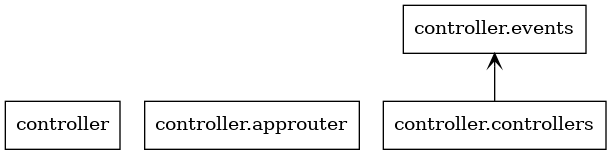
\includegraphics[scale=0.3]{img/controller.png}
      \caption{Structure du contrôleur}
    \end{figure}
  \end{center}

  \begin{block}{Le routeur}
    \begin{itemize}
    \item \textsc{AppRouter} contrôle l'application.
    \item Chaque contrôleur est un état de \textsc{AppRouter}.
    \item Utilisation du \textit{Design Pattern State}.
    \end{itemize}
    
  \end{block}
\end{frame}

\begin{frame}[fragile]{Exemple de contrôleur}
  \footnotesize
  \begin{minted}{python}
    class MainController(Controller):
    def __init__(self):
        super().__init__()
        self._player_info = []
        self._play_ctrl = PlayController(self)
        self._setup_ctrl = SetupController(self)
        self._report_ctrl = ReportController(self)

    def on_event(self, event):
        if event.get('action') == 'S':
            self.on_save()

        if event.get('action') == 'C':
            self.on_load()

        if event.get('action') == 'R':
            self._router.set_controller(self._report_ctrl)

    # ...
  \end{minted}
\end{frame}

\begin{frame}[fragile]{Interactions avec l'utilisateur}
  \footnotesize
  \begin{minted}{python}
    class UserInteractor(ABC):
        @abstractmethod
        def ask(self, msg):
            pass

        @abstractmethod
        def tell(self, msg):
            pass
        
        
    class ConsoleUserInteractor(UserInteractor):
        def ask(self, msg):
            if msg == '\\quitter':
            raise StopAndSave()
            return input(msg)
        
        def tell(self, msg):
            print(msg)

        # ...
  \end{minted}
\end{frame}

\begin{frame}[fragile]{Exemples d'interactions}
  \begin{minted}{python}
    self._view.io().tell(f'\nMatch: {pair[0].name} '
                         f'contre {pair[1].name}')
    res = self._view.io().ask('Résultat du match '
                              f'(0: {pair[0].name}, '
                              f'1: {pair[1].name}, '
                              '2: match nul): ')
  \end{minted}
\end{frame}

\begin{frame}[fragile]{Instanciation des composants}
  \footnotesize
  \begin{minted}{python}
    if __name__ == '__main__':
        user_interactor = ConsoleUserInteractor()
        factory = XMLFactory(user_interactor)
        view = factory.load_from_file('data/menu.xml')
        datastore = TinyDBStore()
        model = ChessClub(datastore)
        
        router = AppRouter(user_interactor, model, view)
        router.set_error_manager(PrintErrorManager(user_interactor))
        router.set_controller(MainController())
        
        try:
            router.run()
        except KeyboardInterrupt:
            print()
            model.quit()
  \end{minted}
\end{frame}

\subsection{Domaine métier}

\begin{frame}[fragile]{Système Suisse des tournois}
  \footnotesize
  \begin{minted}{python}
class PairGenerator(ABC):
    @abstractmethod
    def generate(self, tournament):
        pass


class SwissPairGenerator(PairGenerator):
    def __init__(self):
        pass

    def generate(self, tournament):
        if tournament.is_first_round():
            return self._generate_first_round(tournament)
        return self._generate(tournament)
  \end{minted}
\end{frame}

\begin{frame}[fragile]{Système Suisse des tournois: premier tour}
  \footnotesize
  \begin{minted}{python}
def _generate_first_round(self, tournament):
    players = copy.deepcopy(tournament.players)
    result = []

    players.sort(key=lambda p: int(p.ranking))

    i = 0
    total = int(len(players)/2)

    while i < total:
        result.append((players[i], players[total + i]))
        i += 1

    return result
  \end{minted}
\end{frame}

\begin{frame}[fragile]{Système Suisse des tournois: tours suivants}
  \tiny
  \begin{minted}{python}
def _generate_from_scores(self, tournament, player_scores):
    players = copy.deepcopy(tournament.players)
    result = []

    players.sort(reverse=True, key=lambda p: player_scores[p.name])

    while len(players) > 0:
        p0 = 0
        p1 = 1

        my_round = tournament.previous_round()
        if my_round is not None:
            while True:
                matches = tournament.find_matches_by_players(players[p0],
                                                             players[p1])
                if len(matches) > 0:
                    p1 += 1
                else:
                    break

        result.append((players[p0], players[p1]))

        del players[p0]
        del players[p1 - 1]

    return result
  \end{minted}
\end{frame}

\begin{frame}{Persistance}
  \begin{block}{Principes}
    \begin{itemize}
    \item Un \textsc{DataStore} est un objet capable de
      \begin{itemize}
      \item stocker,
      \item sauvegarder et
      \item charger les données importantes du système.
      \end{itemize}
    \item \textsc{InMemoryStore} $\rightarrow$ garde tout en mémoire
      durant l'exécution du programme.
    \item \textsc{TinyDBStore} $\rightarrow$ travaille avec une base
      de données via TinyDB.
    \end{itemize}
  \end{block}
\end{frame}

\begin{frame}[fragile]{Persistance}
  \tiny
  \begin{minted}{python}
    class DataStore(ABC):
    def __init__(self):
        self._players = []
        self._tournaments = []

    @abstractmethod
    def save(self):
        pass

    @abstractmethod
    def load(self):
        pass

    def store_player(self, player):
        self._players.append(player)

    def store_tournament(self, tournament):
        self._tournaments.append(tournament)

    def players(self):
        return self._players

    def tournaments(self):
        return self._tournaments

    def find_players_by_ranking(self, ranking):
        return [p for p in self._players if int(p.ranking) == int(ranking)]

    def find_players_by_name(self, name):
        return [p for p in self._players if p.name == name][0]

  \end{minted}
\end{frame}

\begin{frame}[fragile]{Persistance: sérialisation d'un match}
  \footnotesize
  \begin{minted}{python}
    @property
    def __dict__(self):
        return {
            'player_0': self._player_0.name,
            'player_1': self._player_1.name,
            'result': int(self._result)
        }
  \end{minted}
\end{frame}

\begin{frame}[fragile]{Persistance: sérialisation d'un tour}
  \footnotesize
  \begin{minted}{python}
    @property
    def __dict__(self):
        result = {
            'name': self._name,
            'start': str(self._start),
            'end': str(self._end),
            'matches': []
        }

        for m in self._matches:
            result['matches'].append(m.__dict__)

        return result
  \end{minted}
\end{frame}

\begin{frame}[fragile]{Persistance: sérialisation d'un tournoi}
  \footnotesize
  \begin{minted}{python}
    @property
    def __dict__(self):
        result = {}
        result['name'] = self._name
        result['place'] = self._place
        result['start_date'] = str(self._start_date)
        result['end_date'] = str(self._end_date)
        result['category'] = self._category
        result['description'] = self._description
        result['players'] = [p.name for p in self._players]

        rounds = []
        for r in self._rounds:
            rounds.append(r.__dict__)
        result['rounds'] = rounds
        result['current_round'] = self._current_round

        return result
  \end{minted}
\end{frame}

\begin{frame}[fragile]{Sauvegarde}
  \footnotesize
  \begin{minted}{python}
        def save(self):
        player_table = self._db.table('Player')
        player_table.truncate()
        for player in self._players:
            player_table.insert(player.__dict__)

        tournament_table = self._db.table('Tournament')
        tournament_table.truncate()
        for tournament in self._tournaments:
            tournament_table.insert(tournament.__dict__)
  \end{minted}
\end{frame}

\begin{frame}[fragile]{Chargement: les joueurs}
  \footnotesize
  \begin{minted}{python}
    def load(self):
        player_table = self._db.table('Player')

        for p in player_table.all():
            self.store_player(Player(
                p['last_name'],
                p['first_name'],
                p['date_of_birth'],
                p['gender'],
                p['ranking']
            ))

        tournament_table = self._db.table('Tournament')
        for t in tournament_table.all():
            # -> suite
  \end{minted}
\end{frame}

\begin{frame}[fragile]{Chargement: les tournois}
  \tiny
  \begin{minted}{python}
            the_tournament = Tournament('', '', '', '', '', '')
            the_tournament._name = t['name']
            the_tournament._place = t['place']
            the_tournament._start_date = t['start_date']
            the_tournament._end_date = t['end_date']
            the_tournament._category = t['category']
            the_tournament._description = t['description']
            the_tournament._current_round = t['current_round']

            for name in t['players']:
                the_tournament.add_player(self.find_players_by_name(name))

            for r in t['rounds']:
                # -> suite
  \end{minted}
\end{frame}

\begin{frame}[fragile]{Chargement: les tours et les matchs}
  \footnotesize
  \begin{minted}{python}
    the_round = Round(r['name'],
                      datetime.date(*[
                          int(i)
                          for i in r['start'].split('-')
                      ]),
                      datetime.date(*[
                          int(i)
                          for i in r['end'].split('-')
                      ]))

    for match in r['matches']:
        m = Match(self.find_players_by_name(match['player_0']),
                  self.find_players_by_name(match['player_1']))
        m.set_result(int(match['result']))
        the_round.add_match(m)

    the_tournament.add_round(the_round)

self._tournaments.append(the_tournament)
  \end{minted}
\end{frame}



\section{Démonstration}
\begin{frame}{Démonstration}
  \begin{block}{Fonctionnalités clefs}
    \begin{enumerate}
    \item Création et exécution d'un tournoi
    \item Mise-à-jour du classement
    \item Génération d'un rapport
    \item Sauvegarde et chargement à tout moment
    \end{enumerate}
  \end{block}
\end{frame}


\section{Conclusion}
\begin{frame}{Conclusion}
  
\end{frame}

% enjeux

% limites
%% pas testé sous MacOS

% extensions
%% suppression d'un joueur
%% interface graphique
%% export des rapports


\begin{frame}{Merci de votre attention}
  \setcounter{tocdepth}{32}
  \tableofcontents
\end{frame}

\end{document}
